\documentclass{article}
\usepackage{graphicx}
\usepackage{amsmath}
\usepackage{hyperref}

\begin{document}

\title{Solutions to hw4 homework on Convex Optimization https://web.stanford.edu/class/ee364a/homework.html}
\author{Andrei Keino}
\maketitle
% from 
% https://www.studocu.com/en-us/document/stanford-university/convex-optimization-i/assignments/2020-hw4sol-hw4/7518536/view
% 5.1, 5.3, 5.12, A3.3, A3.10, A3.32 
\section*{5.1}
A simple example. Consider the optimization problem 
\begin{align*}
&minimize \qquad x^2 + 1 \\
&subject \; to  \qquad (x - 2)(x - 4) \leq 0
\end{align*} 
with variable $x \in R$\\

(a) Analysis of primal problem. Give the feasible set, the optimal value, and the optimal solution.\\

(b) Lagrangian and dual function. Plot the objective
$x^2 + 1$ versus $x$. On the same plot,
show the feasible set, optimal point and value, and plot the Lagrangian $L(x, \lambda)$ versus $x$ for a few positive values of $\lambda.$ Verify the lower bound property $(p^* \leq \inf_x L(x, \lambda) \;for\; \lambda \geq 0 ).$ Derive and sketch the Lagrange dual function $g$. \\

(c) Lagrange dual problem. State the dual problem, and verify that it is a concave maximization problem. Find the dual optimal value and dual optimal solution $\lambda ^*$. Does strong duality hold? \\

(d) Sensitivity analysis. Let $p^*(u)$ denote the optimal value of the problem 
\begin{align*}
&minimize \qquad x^2 + 1 \\
&subject \; to  \qquad (x - 2)(x - 4) \leq u
\end{align*} 
as a function of the parameter $u.$ Plot $p^*(u).$ 
Verify that $dp^*(0) / du = - \lambda^*.$ \\

Solution: \\

(a)\\

The feasible set is $x \in [2, 4] $. The optimal solution is 
$x^* = 2$, the optimal value is $p^* = 5.$ \\

(b)\\
% https://www.latex-tutorial.com/tutorials/figures/
\begin{figure}[h!]
	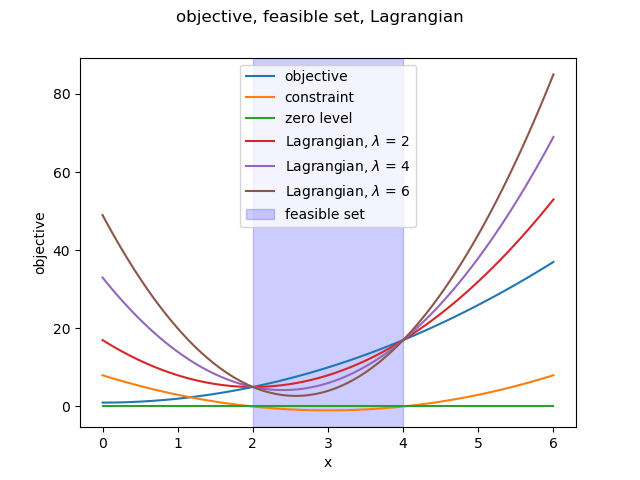
\includegraphics[width=\linewidth]{5_1_b_1.png}
	\caption{objective, feasible set, lagrangian for this problem.}
	\label{fig:5_1_b_1}
\end{figure}

It's easy to see from the Figure 1, that the Lagrangian values on the feasible set are less or equal than the objective values on the feasible set, 
i. e. \\ 
$(p^* \geq \inf_x L(x, \lambda) \;for\; \lambda \geq 0 ).$ \\

(c)\\
The dual objective function for this problem can be found solving the constrained equation for the Lagrangian: \\

\begin{align*}
&g(\lambda) = inf_{x} (x^2 + 1 + \lambda (x - 2)(x - 4))\\
&subject \; to  \qquad \lambda \geq 0
\end{align*} 

The Lagrangian reaches its minimum at the point 
$\tilde x = \frac{3 \lambda}{\lambda + 1}.$
Then the dual objective itself is: \\
$$g(\lambda) = - \lambda + 10 - \frac{9}{(\lambda + 1)}$$ \\
The second derivative of the dual function is:\\
$$g^{''}(\lambda) = - 18 / (\lambda + 1)^3$$
which is obviously less than zero for $\lambda \geq 0,$ i.e. the dual function is concave for $\lambda \geq 0.$


\begin{figure}[h!]
	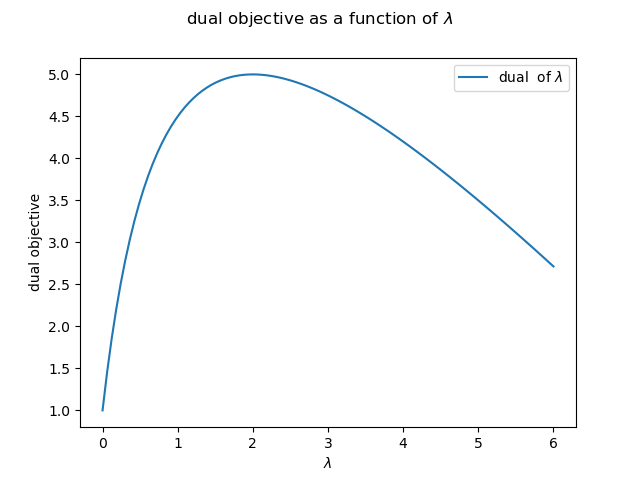
\includegraphics[width=\linewidth]{5_1_b_2.png}
	\caption{Dual objective for this problem.}
	\label{fig:5_1_b_2}
\end{figure}

The dual optimal value $\lambda ^*$ can be found solving the dual problem for the $g(\lambda):$
\begin{align*}
&maximize \qquad g(\lambda) \\
&subject \; to  \qquad \lambda \geq 0
\end{align*} 

or 
\begin{align*}
&d g(\lambda) / {d \lambda} = 0 \\
&subject \; to  \qquad \lambda \geq 0
\end{align*} 

Solving the equation we found $\lambda ^* = 2;$ optimal value of $g$ (i.e. $sup_\lambda \{g(\lambda)\}$) $g^* = 5.$
We can see that $p^* = 5 = g^*,$ i. e. strong duality holds.\\

(d) \\

Solving the constraints equation $(x - 2)(x - 4) = u$ we get:\\
$x_{1, 2} = 3 \pm \sqrt{1 + u}, \; u \geq 1.$ Then \\

\begin{equation}
p^*(u) =
\begin{cases}
	\text{not exists},			& \text{if } u < -1 \\
	u - 6 \sqrt{1 + u} + 11, 	& \text{if } - 1 \leq u \leq 8  \\
	1, 							& \text{if } u > 8
\end{cases}       
\end{equation}

\begin{figure}[h!]
	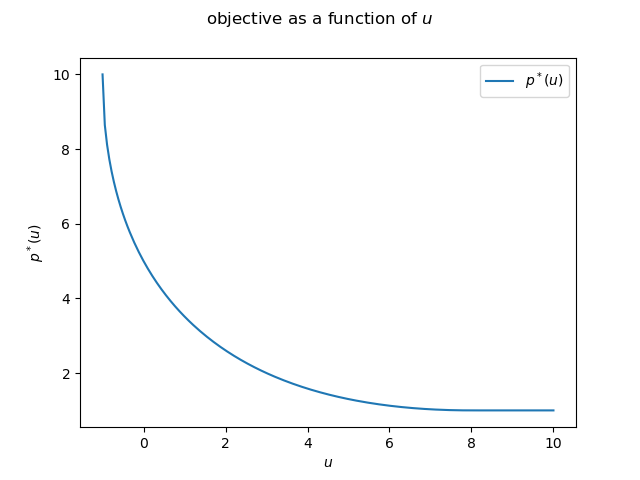
\includegraphics[width=\linewidth]{5_1_3.png}
	\caption{Graph of $p^*(u)$ for this problem.}
	\label{fig:5_1_3}
\end{figure}

And finally:
$$dp^*(u) / du = 1 - \frac{3}{\sqrt{1 + u}}$$
Then $dp^*(0) / du = -2 = - \lambda^*$

\section*{5.3}

Problems with one inequality constraint. Express the dual problem of 
\begin{align*}
&\text{minimize }  c^Tx \\
&\text{subject to }  f(x) \leq 0
\end{align*} 
with $c \neq 0$ in terms of the conjugate $f^*.$ Explain why the problem you give is convex. We do not assume $f$ is convex. \\

Solution: \\
The dual problem of the task is:
\begin{align*}
&\text{maximize }  \inf_x (c^Tx + \lambda f(x)) \\
&\text{subject to }  \lambda \geq 0
\end{align*} 
The definition of the conjugate function is:
$$ f^*(y) = \sup_x (y^T x - f(x)) = - \inf_x(f(x) - y^Tx)$$\\
i.e. the dual problem can be reformulated as:

\begin{align*}
&\text{maximize }  F(c, \lambda) \\
&\text{subject to }  \lambda \geq 0
\end{align*} 
where $F(c, \lambda) = - \lambda f^*(-c/\lambda), $
where $f^*$ is the conjugate function of $f,$ and it is always convex.  $F(c, \lambda)$ is the concave function, as it is the negative perspective of the convex function $f^*$.

\section*{5.12}
Analytic centering. Derive a dual problem for 
$$\text{minimize } - \sum_{i = 1}^{m} log(b_i - a_i^T x)$$
with domain 
$\{x\; | \;  a_i^T x \leq b_i, \; i = 1, ..., m\}.$ First introduce new variables $y_i$ and equality constraints $y_i = b_i - a_i^T x.$ (The solution of this problem is called the analytic center of the linear inequalities $a_i^T x \leq b_i, \; i = 1, ..., m\}.$ 
Analytic centers have geometric applications and play an
important role in barrier methods. \\

Solution:

This problem is equivalent to:
\begin{align*}
\text{minimize } \qquad & - \sum_{i = 1}^{m} log(y_i) \\
\text{subject to } \qquad &y + A^T x - b = 0 \\
\end{align*}

where the matrix $A$ composed from the rows $a_i^T.$ \\
Then the Lagrangian is\\
$$
L(x, y, \nu) = - \sum_{i = 1}^{m} log(y_i) + 
\nu^T(y + A^T x - b)
$$
The dual function is
$$
g(v) = \inf_{x, y}( - \sum_{i = 1}^{m} log(y_i) + 
\nu^T(y + A^T x - b))
$$

The term $\nu^TA^Tx$ is unbounded below as 
$x \rightarrow \infty,$ so \\

\begin{equation*}
g(\nu) =
\begin{cases}
\sum_{i = 1}^{m} log(y_i) + m - \nu^T b , 	
& \nu^TA^T = 0, \; \nu_i \geq 0  \\
- \infty, 					& \nu^TA^T \neq 0 
\end{cases}       
\end{equation*}

and the dual problem is:

\begin{align*}
\text{maximize } \qquad 
& \sum_{i = 1}^{m} log(\nu_i) + m - \nu^T b \\
\text{subject to } \qquad & \nu^TA^T = 0
\end{align*}


\end{document}

